\chapter{Návrh desky plošných spojů}

Deska plošných spojů byla navržena podle výrobních pravidel firmy JLCPCB\footnote{https://jlcpcb.com/}. Maximální rozměry jsou $\SI{100}{}\times \SI{100}{\milli\metre}$ a byla využita dvouvrstvá deska. Do těchto výrobních možností je tedy nutné koncipovat celý návrh desky plošných spojů. Osazování proběhne v drtivé většině součástek u dříve zmíněné firmy strojně, jelikož i za cenu včetně osazení je cena součástek nakoupená právě u nich nesrovnatelná například s českou konkurencí. Jednou z možných nevýhod je absence strojního osazení z obou stran desky, tento výrobce umožňuje osazovat pouze jednu stranu desky plošného spoje.

Pro dosažení co nejlepších parametrů celého obvodu bylo dbáno na doporučené zapojení dle datasheetu výrobců. Největší pozornost byla věnována oblasti spínaného zdroje, jelikož zde je důležité správně rozložit součástky a dimenzovat spoje na desce. Na obrázku \ref{fig_PCB-top} je vidět celá navržená deska plošných spojů o rozměrech $\SI{100}{}\times \SI{100}{\milli\metre}$ z horní strany. Výsledná deska plošných spojů byla navržena v programu KiCad\footnote{https://www.kicad.org/}, který je dostupný zdarma a lze jej používat i pro komerční projekty.

\begin{figure}[h]
    \centering
    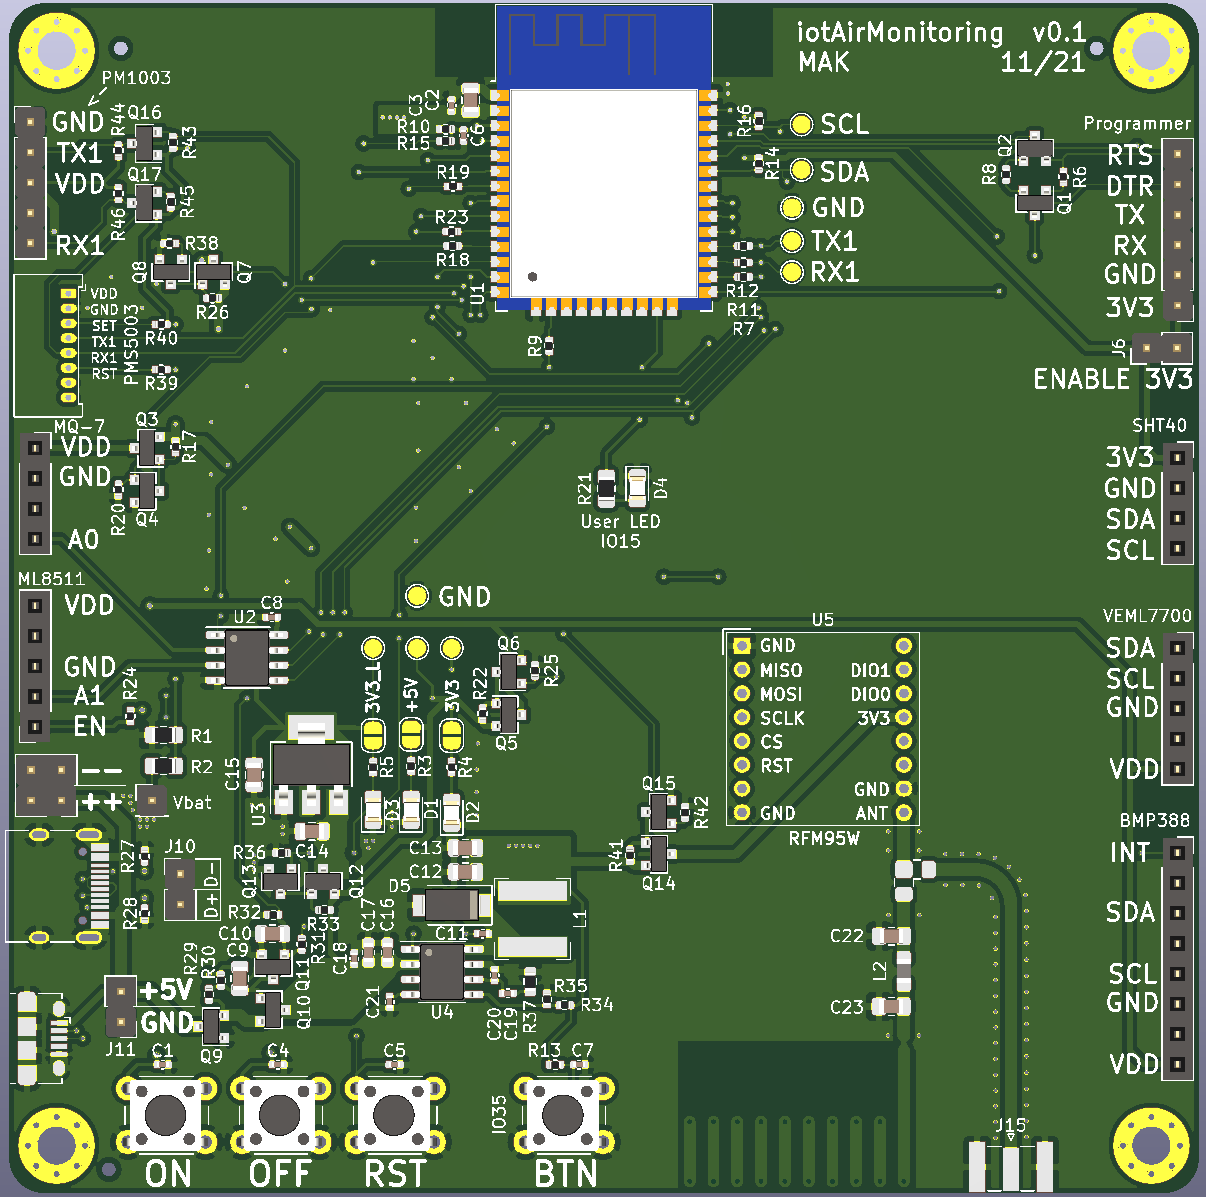
\includegraphics[width=0.7\textwidth]{obrazky/PCB_top.png}
    \caption{Pohled na 3D model desky plošného spoje shora.}
    \label{fig_PCB-top}
\end{figure}